\documentclass{article}
\usepackage[utf8]{inputenc}
\usepackage{geometry}
\usepackage{longtable}
\usepackage{graphicx} % For including images
\usepackage{hyperref} % For hyperlinks

\geometry{
 a4paper,
 total={170mm,257mm},
 left=20mm,
 top=20mm,
}

\title{Software Architecture of Train Inter Payment System (TrIP)}
\author{Group 04}
\date{\today}

\begin{document}

\maketitle
\newpage

\section*{Product Introduction}
The Train Inter Payment System (TrIP) is a collaborative project initiated by three railroad tycoons to streamline the payment process for train travel. These tycoons, operating a network connecting towns, industries, and a university, aim to address the interoperability issues of their existing payment systems. TrIP will feature smart payment terminals at each station, enabling direct communication for subscription validation or single-fare payments. This system, underpinned by a service-based architecture, involves critical components like payment terminals and tycoon-specific systems. It's designed with key stakeholder requirements in mind: maintainability and operational efficiency for the owner, usability and reliability for the tycoons, and usability and security for passengers. The project seeks to ensure passengers can easily manage payments and subscriptions across the network, enhancing the overall travel experience while safeguarding user data.

\newpage
\subsection{Decision 1: UI}

\subsection*{Status}
Accepted.

\subsection*{Architectural Summary}
% TODO

\subsection*{Concern}
Passengers require a user interface that is easy to navigate, visually appealing, and provides a seamless experience across different tycoon systems.

\subsection*{Context}
In the context of designing an intuitive and engaging user interface for the TrIP system terminals, we face the challenge of selecting guiding principles and frameworks that will shape the user experience and interaction design.
The design of the user interface on the terminals involves the passenger's interaction with the system, from querying routes to finalizing ticket purchases. It is an essential component of the system that directly affects user satisfaction and system usability.

\subsection*{Criteria}
The decision will be guided by the following criteria:
\begin{itemize}
    \item Consistency in design to provide a unified look and feel across all terminals.
    \item Accessibility to ensure the system is usable by all passengers, including those with disabilities.
    \item Responsiveness so that the interface can adapt to various screen sizes and orientations.
    \item Ease of maintenance and scalability for future enhancements.
    \item Alignment with the latest trends in user interface design and technology.
\end{itemize}

\subsection*{Option 1: Use of Standardized UI Components}
This approach involves adopting a comprehensive design system, such as Google's Material Design or IBM’s Carbon Design System, which offers a robust set of standardized UI components. These components include buttons, forms, toggles, navigation patterns, and more, all designed with consistency and usability in mind. By utilizing these pre-designed components, the development process can be significantly accelerated, as developers and designers will not need to create common UI elements from scratch. This ensures a cohesive look and feel across the entire application, enhancing the user's ability to intuitively navigate the system.
\begin{itemize}
    \item \textbf{Pro:} Significantly reduces development time and ensures UI consistency.
    \item \textbf{Pro:} Both Google's Material Design and IBS's Carbon Design System are open source, hence they would allow developers to easily debug the interface, identify possible bugs, seek for contributions online or even contribute themselves.
    \item \textbf{Con:} May limit unique branding opportunities and design customization. 
    \item \textbf{Con:} Some developers may consider it a limit for their creativity. 
\end{itemize}

\subsection*{Option 2: Custom Designed Interactive Interfaces}
This option focuses on creating bespoke interactive interfaces from the ground up, specifically tailored to the unique needs and brand identity of the TrIP system. This could involve developing custom animations, unique layout designs, and interactive elements that engage users in a novel way. By focusing on custom designs, the TrIP system can distinguish itself from competitors and provide a unique user experience that directly addresses specific user needs and preferences.
\begin{itemize}
    \item \textbf{Pro:} Allows for full creative freedom and the opportunity to innovate.
    \item \textbf{Pro:} Less operational cost, and higher maintainability.
    \item \textbf{Con:} More time-consuming and expensive due to the bespoke nature of the design and development process.
    \item \textbf{Con:} Expertise within the developing team is needed, possibly more developers. This might offset the lower operational cost.
\end{itemize}

\subsection*{Option 3: Open Source Frameworks}
Utilizing open-source UI frameworks such as Bootstrap, Foundation, or Vue.js offers a middle ground between complete customization and strict standardization. These frameworks are supported by large communities of developers, ensuring that the frameworks are well-documented, frequently updated, and robust against common web development challenges. They come with a variety of UI components that can be easily modified to fit the system’s needs, providing both speed in development and a degree of customization.
\begin{itemize}
    \item \textbf{Pro:} Combines rapid development with the flexibility of customization.
    \item \textbf{Con:} Might still require significant effort to stand out from the default "framework look."
    \item \textbf{Con:} Possible discontinuation.
\end{itemize}

\subsection*{Option 4: Proprietary High-End Frameworks}
Choosing proprietary frameworks such as Telerik, DevExpress, or Adobe XD’s design systems offers access to a suite of advanced features, including sophisticated data visualization tools, complex UI components, and comprehensive support services. These frameworks are often optimized for performance and come with extensive documentation and professional support, ensuring that the development team can create a high-quality user interface while potentially saving time on troubleshooting and problem-solving.
\begin{itemize}
    \item \textbf{Pro:} Provides a wide range of advanced features and dedicated support.
    \item \textbf{Con:} Incurs additional costs due to licensing fees and may lock the project into a specific vendor or technology stack.
    \item \textbf{Con:} Train system doesn't have to be that compilicated, high-end products can be redundant, also the passengers want us to keep it simple.
\end{itemize}

\subsection*{Decision}
Option 1 is chosen. This option lifts a lot of weight from the development team. This reduces operational cost and enhances maintenability, which are the main concerns of the TrIP owner. Furthermore, these interfaces are well tested and user-friendly, making them a natural choice to satisfy the need for usability of the passengers and the reliability requested by the tycoons. 
Generally speaking, user interfaces for train systems are not sophisticated enough to require more expensive and complicated set-ups. 
A careful user testing is strongly adviced, to choose a suitable setup.

\subsection*{Consequences}
\textbf{Positive Consequences:}
\begin{itemize}
    \item Access to a broad community for support and troubleshooting.
    \item Cost savings by avoiding licensing fees associated with proprietary software.
    \item Rich ecosystem of plugins and extensions to enhance functionality.
    \item Frequent updates and a large pool of developers familiar with the frameworks.
\end{itemize}
\textbf{Negative Consequences:}
\begin{itemize}
    \item Potential dependency on external communities for critical updates and support. Some of these might require expensive professional support.
    \item Risk of choosing a framework that may not align with long-term technology trends or become obsolete. Information sourcing about the future of the chosen project is crucial.
    \item Need for rigorous selection to ensure accessibility and responsiveness standards are met. This would be a consequence of any of the choices listed.
\end{itemize}


\newpage
\subsection{Decision 2: Database technology}

\subsection*{Status}
Accepted.

\subsection*{Architectural Summary}
% TODO

\subsection*{Concern}
The main concern lies in selecting a database that can efficiently manage complex data relationships, provide high transactional integrity, and scale as needed without compromising on performance or security.

\subsection*{Context}
In developing the TrIP system, tasked with unifying the payment and subscription management across three railroad tycoons' operations, we are faced with the decision of choosing an appropriate database technology. This choice hinges on our need to ensure data integrity, support complex queries for transaction processing, and maintain scalability and security.
The database must handle a wide array of data, including user subscriptions, fare transactions, and station and route information, necessitating a robust system that supports complex queries and relational data structuring.
The architecture might include more than one databases, depending on the needs that will arise during later decisions.

\subsection*{Criteria}
\begin{itemize}
    \item Data integrity and transactional consistency for financial transactions.
    \item Ability to support complex queries and relational data models.
    \item Scalability to grow with the system's user base and data volume.
    \item Performance under varying load conditions.
    \item Comprehensive security features to safeguard sensitive data.
\end{itemize}

\subsection*{Option 1: SQL Database (e.g., PostgreSQL)}
A relational database model renowned for its strong consistency, ACID (Atomicity, Consistency, Isolation, and Durability) compliance, and the ability to efficiently handle complex queries and data relationships.
\begin{itemize}
    \item \textbf{Pro:} High data integrity and robust support for complex relational data structures.
    \item \textbf{Pro:} We have a highly structured data.
    \item \textbf{Pro:} More developers are familiar with it, more resources on the topic. It has a strong community and over 30 years of active development.
    \item \textbf{Pro:} Good with concurrency.
    \item \textbf{Pro:} Open source and free.
    \item \textbf{Con:} Scalability challenges in horizontally distributed architectures compared to NoSQL options.
    \item \textbf{Con:} Requires accurate upfront planning of the data model due to its structured nature, thereby limiting flexibility.
\end{itemize}

\subsection*{Option 2: NoSQL Database (e.g., MongoDB)}
A distributed database system designed for scalability and flexibility, suitable for handling large volumes of diverse data types.
\begin{itemize}
    \item \textbf{Pro:} Offers superior scalability and flexibility for managing unstructured or semi-structured data.
    \item \textbf{Pro:} Enhances performance for non-structured data.
    \item \textbf{Con:} May compromise transactional integrity and consistency in favor of performance and scalability.
\end{itemize}

\subsection*{Decision}
After thorough consideration, the decision is to implement an \textbf{SQL database}, specifically PostgreSQL for it being open source, for the TrIP system. This decision is underpinned by the SQL database's unmatched data integrity, support for complex transactions, and relational data modeling capabilities, which are crucial for the financial transactions and data relationships inherent in the TrIP system. Furthermore, train payment data are by nature very structured, don't give much creativity to the passengers, thus a relational database seems a more natural choice. Given the higher familiarity of developers, this choice is good for the QAs favoured by the TrIP owner, such as:
\begin{itemize}
    \item Maintainability (priority 2). The owner wants a minimum amount of effort to maintain and build the system
    \item Operational costs (priority 2). The operational costs of the system should be as low as possible.
\end{itemize}

\subsection*{Consequences}
\textbf{Positive Consequences:}
\begin{itemize}
    \item Ensures high levels of data integrity and transactional consistency, critical for financial data and user subscriptions.
    \item Facilitates complex data queries and relationships, enabling sophisticated data analysis and reporting.
    \item Provides robust security features to protect sensitive data and comply with data protection regulations.
\end{itemize}
\textbf{Negative Consequences:}
\begin{itemize}
    \item May require additional strategies for scaling horizontally, such as implementing read replicas or sharding, to manage large data volumes and high traffic loads effectively.
    \item Could necessitate more intensive resource management and optimization to ensure performance at scale.
\end{itemize}
Choosing an SQL database aligns with the TrIP system's core requirements for data integrity, relational data handling, and transactional consistency. This foundation will support the system's initial functionality and long-term growth, with a focus on maintaining data accuracy and trustworthiness.
\newpage
\subsection{Decision 3: Routes management}

\subsection*{Status}
Accepted.

\subsection*{Architectural Summary}
% TODO

\subsection*{Concern}
The concern is to facilitate a seamless travel planning experience for passengers by ensuring the system can accurately and efficiently gather available route options from various tycoon systems and present them based on the user's criteria of price, time, and subscription status.

\subsection*{Context}
In the context of enhancing the TrIP system's ability to provide optimized travel options, we face the challenge of efficiently querying multiple tycoon systems to gather route information that aligns with passenger preferences and existing subscriptions.
The decision is centered on the system's interface with tycoon systems to retrieve and optimize route data, which impacts the functionality and performance of the terminal's route planning features for the passengers.

\subsection*{Criteria}
The key criteria for the decision include:
\begin{itemize}
    \item User-friendly passenger interface.
    \item Comprehensive and diverse route options.
    \item Accurate representation of options based on multiple factors.
    \item Streamlined integration with multiple tycoon systems.
\end{itemize}

\subsection*{Option 1: Direct Tycoon Integration}
Terminals directly interface with each tycoon system and the central database to collate route options. The route optimizer processes this data to present optimal travel solutions. This requires our system to have APIs to query each of the tycoons systems.
\begin{figure}[ht]
    \centering
    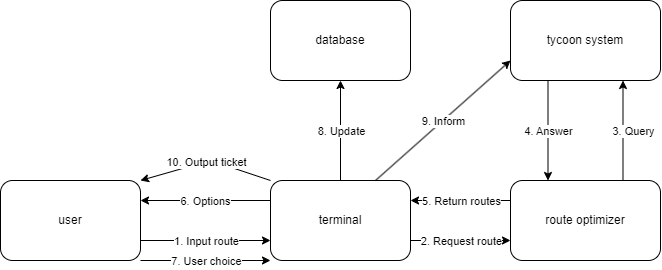
\includegraphics[width=\textwidth]{drawings/decision3_drawings/direct.png}
    \caption{Direct Data Management Interface}
    \label{fig:direct-data-interface}
\end{figure}

\subsection*{Option 2: Centralized Route Management Module}
A central route data management module acts as an intermediary between terminals and tycoon systems, standardizing and aggregating data before it is processed by the route optimizer. A database containing the timetables will be kept up to date by the tycoon (possibly though an API, this will be the focus of a later decision). The route data management system might cache optimized routes, in order to minimize database requests. A module specialized in running optimizations with the data it is provided with interacts solely with the Route Management Module.
\begin{figure}[ht]
    \centering
    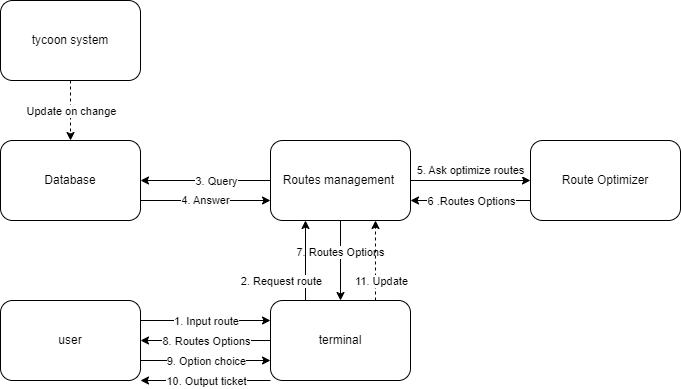
\includegraphics[width=\textwidth]{drawings/decision3_drawings/centralized.png}
    \caption{Centralized Route Management Module. Dashed lines represents steps to be explained in future decisions.}
    \label{fig:centralized-data-interface}
\end{figure}
  
\subsection*{Decision}
We have decided to proceed with Option 2: Centralized Route Management Module. This decision is based on the module's ability to simplify the data flow between systems and to effectively manage the complexity of integrating with multiple tycoon systems. The introduction of a separate data management module will allow for greater flexibility and scalability.

\subsection*{Consequences}
\textbf{Positive Consequences:}
\begin{itemize}
    \item Simplified data flow between the trip system and tycoons.
    \item Improved scalability and maintainability of the system.
    \item Easier to integrate with current and future tycoon systems.
\end{itemize}
\textbf{Negative Consequences:}
\begin{itemize}
    \item Initial development and integration effort for the new module.
    \item Potential complexity in data synchronization between modules.
\end{itemize}
This approach is expected to provide a solid foundation for the system's scalability and adaptability to evolving requirements and stakeholder needs.
\newpage

% \begin{table}[H]
    \resizebox{\textwidth}{!}{%
    \begin{tabular}{|l|c|c|c|c|c|c|c|c|c|c|c|}
    \hline
    \textbf{User Story} & \textbf{Usability} & \textbf{Performance} & \textbf{Security} & \textbf{Modifiability} & \textbf{Deployability} & \textbf{Energy Efficiency} & \textbf{Availability} & \textbf{Safety} & \textbf{Integrability} & \textbf{Testability} & \textbf{Accessibility} \\
    \hline
    1. Frequent traveler monthly pass & + &  &  &  &  &  &  &  &  &  &  \\
    \hline
    2. Check travel card balance & + &  &  &  &  &  &  &  &  &  &  \\
    \hline
    3. Subscription notifications & + &  &  &  &  &  &  &  &  &  &  \\
    \hline
    4. Mobile app management & + &  &  &  & - &  &  &  &  &  &  \\
    \hline
    5. Carbon footprint tracking &  & - &  &  &  & + &  &  &  &  &  \\
    \hline
    6. Accessible services info & + &  &  &  &  &  &  & + &  &  &  \\
    \hline
    7. Voice-activated features & + &  &  & - & - &  &  &  &  &  & + \\
    \hline
    8. Simple interface for elders & + &  &  & + &  &  &  &  &  &  &  \\
    \hline
    9. Multilanguage options & + &  &  & - &  &  &  &  &  &  &  \\
    \hline
    10. Quick access to popular trips & + & - &  & - &  &  &  &  &  &  &  \\
    \hline
    11. Scan student card for benefits & + &  &  & - &  &  &  &  &  &  &  \\
    \hline
    12. Single transaction for subscriptions & + & - &  &  &  &  &  &  &  &  &  \\
    \hline
    13. Charge train cards at terminal & + &  &  & - &  &  &  &  &  &  &  \\
    \hline
    14. Interface for visually impaired & + &  &  &  &  &  &  &  &  &  & + \\
    \hline
    15. Block payment for blocked routes & + & - &  & - &  &  &  &  &  &  &  \\
    \hline
    16. Single ticket across all networks & + & - &  & - &  &  &  &  &  &  &  \\
    \hline
    17. Subscriptions advice for commuting & + & - &  & - &  &  &  &  &  &  &  \\
    \hline
    18. Adherence to security standards &  &  & + & - &  &  &  &  & - & - &  \\
    \hline
    19. Detailed reporting for government & + &  &  & - &  &  &  &  & - &  &  \\
    \hline
    20. Reduced fares for eligible populations & + & - &  & - &  &  &  &  &  &  &  \\
    \hline
    21. Revenue tracking for tycoons & + & - &  & - &  &  &  &  &  &  &  \\
    \hline
    22. Exclusive promotions & + &  &  & - &  &  &  &  &  &  &  \\
    \hline
    23. Payment system integration & + &  &  & - &  &  &  &  & + & - &  \\
    \hline
    24. Access to analytics &  &  &  & - &  &  &  &  & + &  &  \\
    \hline
    25. Assistance for ticket purchases & + &  &  & - &  &  &  &  &  &  &  \\
    \hline
    26. Temporary fare adjustments &  &  &  & - &  & + &  &  &  &  &  \\
    \hline
    27. Integration with maintenance tools &  &  &  & - &  & + &  &  &  &  &  \\
    \hline
    28. Audit trails and compliance &  &  &  & - &  &  &  &  &  &  &  \\
    \hline
    \end{tabular}%
    }
    \caption{User Stories and Quality Attributes}
\end{table}

\section*{Context Viewpoint}
\subsection*{View: \textless{}Name\textgreater{}}
\subsubsection*{Model}
Place here the model representation of the view

\subsubsection*{Description}
Short description of the view

\subsubsection*{Glossary of Elements}
\begin{longtable}{lll}
Id & Name & Description \\
\end{longtable}

\subsection*{Analysis on Perspectives}
Describe how the view satisfies the different perspectives. 

\section*{Functional Viewpoint}

\section*{Information Viewpoint}

\section*{Concurrency Viewpoint}

\section*{Development Viewpoint}

\section*{Deployment Viewpoint}

\end{document}
